\subsection{Protocol and Components}
The following are the network architectures we will be using: \\
\textbf{1. \textunderscore{ESP NOW}} \\
ESP-NOW is a wireless communication protocol based on the data-link layer, which reduces the five layers of the OSI model to only one. This way, the data need not be transmitted through the network layer, the transport layer, the session layer, the presentation layer, and the application layer. Also, there is no need for packet headers or unpackers on each layer, which leads to a quick response reducing the delay caused by packet loss in congested networks. 
\begin{figure}[H]
    \centering
    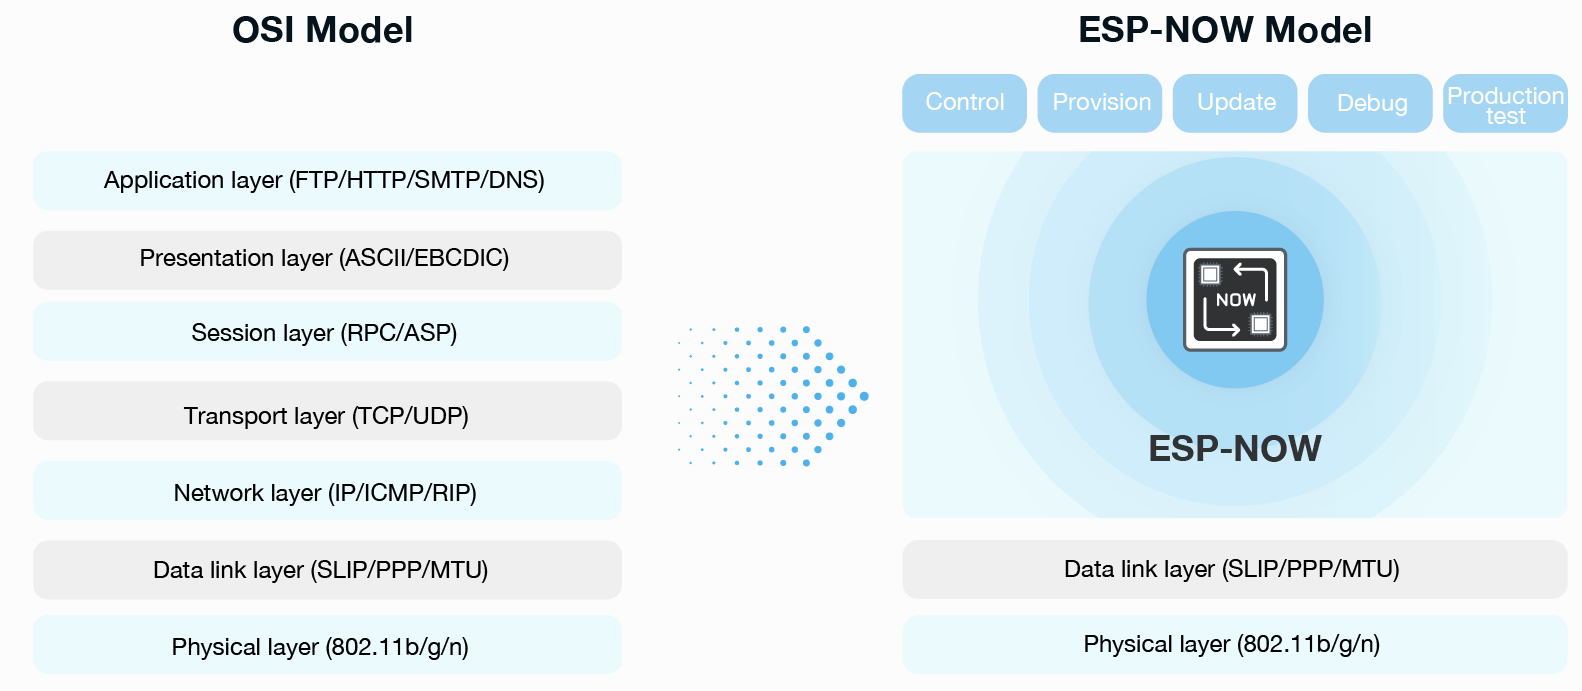
\includegraphics[width=0.75\linewidth]{Files/Images/model-en.png}
    \caption{Comparision of the OSI standard layers and the ESP NOW protocol layers}
    \label{fig:enter-label}
\end{figure}
Here are the key features of the ESP NOW Protocol:
\begin{itemize}
    \item It has a fast and user-friendly pairing method that is suitable for connecting “one-to-many” and “many-to-many” devices, while also controlling them
    \item Occupies fewer CPU and flash resources
    \item Can be used as an independent protocol that helps with device provisioning, debugging, and firmware upgrades
    \item  ECDH and AES algorithms make data transmission more secure
    \item The window synchronization mechanism greatly reduces power consumption
\end{itemize}